%# -*- coding: utf-8-unix -*-
% !TEX program = xelatex
% !TEX root = ../thesis.tex
% !TEX encoding = UTF-8 Unicode

\subsection{基于神经网络的语义匹配模型}
\label{sec:compqa-nn}


%0. present the model in figure xxx: relation matching and entity linking
%1. the main part is RM: model as similarity task
%2. question side: sentential, syntactic
%3. path side: decomposition into parallel parts.
%4. each repr: relation sequence and name sequence.
%5. final score: combination of RM, EL and others.
%6. talk in detail.

本节介绍的语义匹配模型如\figref{fig:compqa-nn}所示。
作为预处理部分,查询图中使用的实体(或时间)节点对应于问句中的短语
被替换为单词$\langle E \rangle$ (或 $\langle Tm \rangle$),
这样问句的语义将不会被具体的实体或年份所干扰。
为了对查询图整体进行编码,
我们首先将其分拆为从答案节点出发,指向不同叶节点的谓词路径,也称为语义成分。
同样为了去除具体的实体、时间、顺序值对语义的干扰,谓词序列不包括叶节点的信息,
类型限制是一个特例,作为模型输入的谓词序列为[ \textit{IsA}, \textit{river} ],
类型节点的信息被包含在内。
接下来将逐个介绍对问句和谓词序列的编码,
基于查询图整体语义表示计算相似度的方式。

%  The architecture of the proposed model is shown in \figref{fig:nn}.
%  %As a preprocessing step, we remove non-semantic information from both the question and the guery graph.
%  We first replace all entity (or time) mentions used in the query graph
%  by dummy tokens $\langle E \rangle$ (or $\langle Tm \rangle$).
%  %as changing ``United States'' to ``China'' doesn't affect the semantic meaning of
%  %our running example.
%  To encode the complex query structure,
%  we split it into predicate sequences starting from answer to focus nodes,
%  which we call \textit{semantic components}.
%  The predicate sequence doesn't include the information of focus nodes,
%  except for type constraints, where we append the focus type to the \textit{IsA} predicate,
%  resulting in the predicate sequence like \{\textit{IsA}, \textit{river}\}.
%  We introduce in detail the encoding methods for questions and predicate sequences,
%  and how to calculate the semantic similarity score.

%利用的信息:字面顺序,依存语法,知识库向量
%The propose neural network encodes both semantic components and questions
%into vector representation using sentential, syntactical and KB structural information.
%Finally the model merges vector representations of different components into 
%a the vector the entire graph,
%and calculate the semantic similarity of the query graph, given the question.


\begin{figure*}[ht]
	\centering
    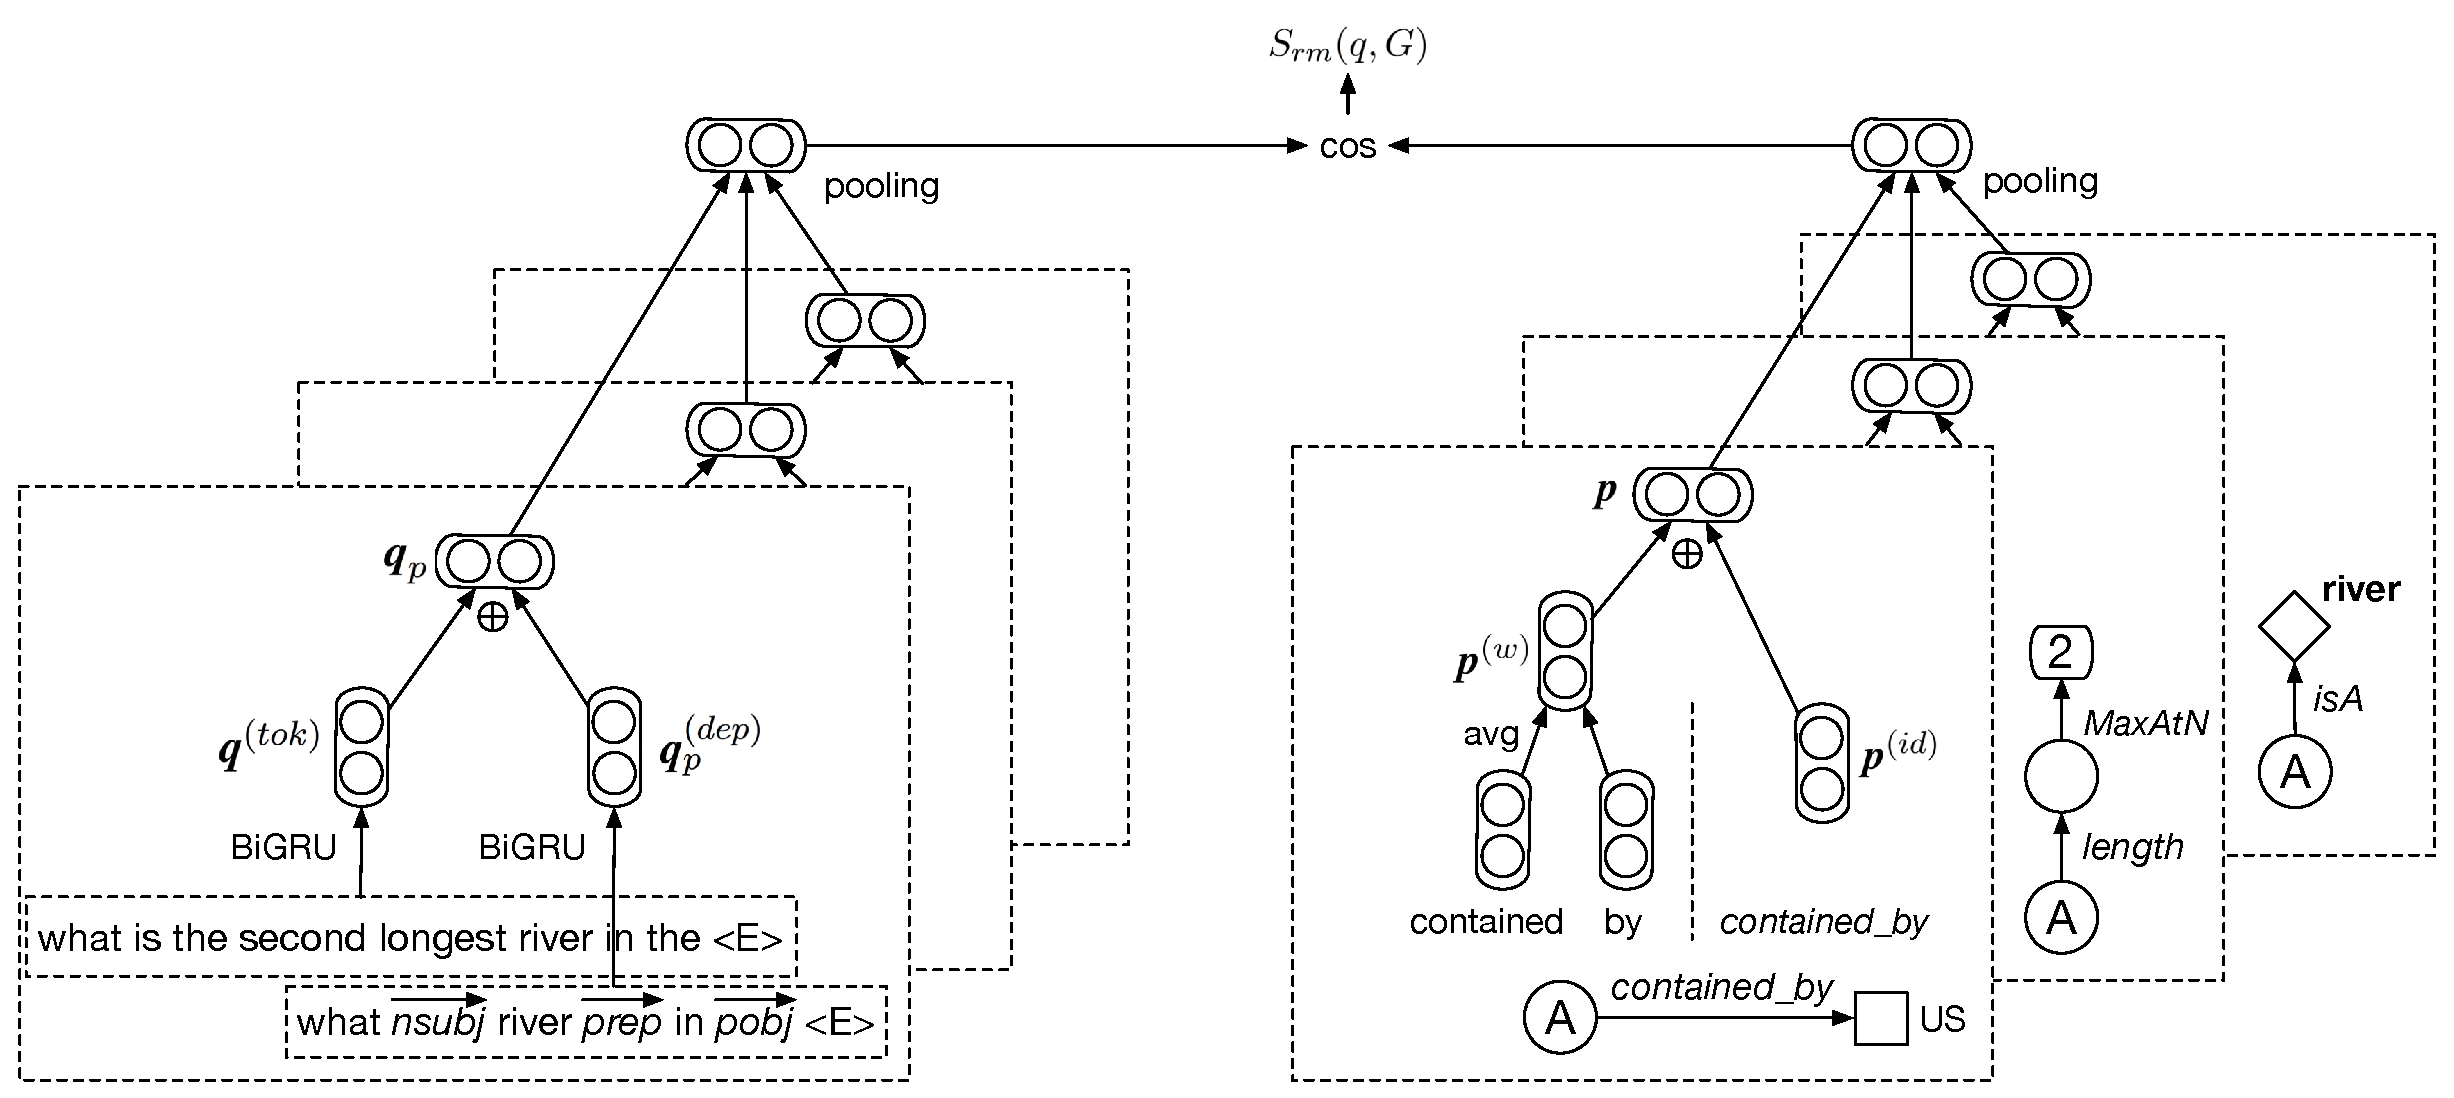
\includegraphics[width=1.0\columnwidth]{figure/compqa/overview.eps}
	\bicaption{语义匹配模型的整体结构}{Overview of proposed semantic matching model.}
	\label{fig:compqa-nn}
\end{figure*}




\subsubsection{语义成分编码}
\label{sec:compqa-schema-encoding}


%In the part of relation matching, we need to encode the query graph.
%To encode the query graph, we first decompose the graph into semantic aspects.
%The semantic aspect is defined as one path in the query graph,
%which starts from the answer node and ends with a leaf node (candidate entities, types, times, ordinals).
%As the example shown in \figref{xxxx},
%the candidate graph is decomposed into 3 semantic aspects which provide the following parallel clues:
%``the answer is in China'',
%``the answer is a river'', 
%``the answer ranks second by descending order of length''.
%The whole query graph represents the combination of clues, representing a complex semantics.


为了对语义成分$p$进行编码,模型对主要利用谓词序列的名字信息,
以及每个谓词在知识库中的编号信息。
以\figref{fig:compqa-nn}为例,查询图的第一个语义成分仅由一个谓词构成,
对应的编号序列为[ \textit{contained\_by} ]。
将序列中的每个谓词在知识库中显示的名字相连,即可的到谓词名字序列,
即[ ``contained'', ``by'' ].

%  To encode a semantic component $p$, we take the sequence of both predicate ids
%  and predicate names into consideration.
%  As the example shown in \figref{fig:nn}, the id sequence of the first semantic component
%  is \{\textit{contained\_by}\}, 
%  and the predicate word sequence is the concatenation of canonical names for each predicate,
%  that is \{``contained'', ``by''\}.
%  %We use both id and labels in the knowlege base to encode each semantic aspect.
%  %Each aspect repred by a sequence of KB predicates and types along the path.
%  %Leave entities, times and ordinal numbers out. (don't care the detail time, number or entities)
%  %Sequence at different granularities.
%  %word sequence of the path: $p^{(w)} = \{p_1^{(w)}, \dots, p_n^{(w)}\}$.
%  %id sequence of the path: $p^{(id)} = \{p_1^{(id)}, \dots, p_m^{(id)}\}$.
%  %(from type.object.name relation.)

%Different methods to encode the path representation given the sequences.

对于语义成分的谓词名字序列$\{p_1^{(w)}, \dots, p_n^{(w)}\}$,
我们首先通过词向量矩阵$E_w \in \mathbb{R}^{|V_w| \times d}$
将原始序列变为词向量$\{\bi{p}_1^{(w)}, \dots, \bi{p}_n^{(w)}\}$,
其中 $|V_w|$表示自然语言词汇数量,
$d$表示词向量维度。
接着我们采用词平均的方式计算整个名字序列的语义向量,即
%  Given the word sequence $\{p_1^{(w)}, \dots, p_n^{(w)}\}$, %we use word embedding matrix to transform words into vectors.
%  we first use a word embedding matrix $E_w \in \mathbb{R}^{|V_w| \times d}$ to convert 
%  the original sequence into word embeddings $\{\bi{p}_1^{(w)}, \dots, \bi{p}_n^{(w)}\}$,
%  where $|V_w|$ denotes the vocabulary size of natural language words,
%  and $d$ denotes the embedding dimension.
%  %TODO: talk later
%  %The word embedding matrix is initialized by publicly available pre-trained results, 
%  %such as Word2vec~\cite{mikolov2013} and GloVe~\cite{xxx}. 
%  Then we represent the word sequence using word averaging:
%  %Then we encode the whole sequence in continuous bag-of-words 
%  %\textbf{Bag-of-Words}:
$\bi{p}^{(w)} = \frac{1}{n} \sum_{i}{\bi{p}_i^{(w)}}$.
%\textbf{Recurrent-Words}: We use GRU~\cite{xx} as the recurrent cell.
%The sequence of word vectors are fed into a bidirectional GRU layer,
%and the repr is the concatenation between the last forward and backward hidden states,
%$\bi{p}^{(w)} = [\overrightarrow{\bi{h}}_n^{(w)};\overleftarrow{\bi{h}}_1^{(w)}]$
对于谓词编号序列$\{p_1^{(id)}, \dots, p_m^{(id)}\}$,
我们将整个序列视为整体,并根据序列级别的向量矩阵$E_p \in \mathbb{R}^{|V_p| \times d}$,
直接转换为语义向量表示,其中$|V_p|$代表训练数据中不同的编号序列数量。
之所以将编号序列看做整体,而不使用编号的向量平均或循环神经层表示语义,
主要原因有以下三点:
1) 根据候选图生成方式,每个语义成分的谓词编号序列长度不超过3;
%so?这可以是不使用RNN的理由,但不是不使用wAvg的理由
2) 通常情况下,对单个谓词序列进行打乱重排操作,新的序列是非法的,不会出现在其它查询图中;
3) 不同的谓词序列数量约等于知识库中不同的谓词数量,不带来成倍增长。
将名字序列和编号序列的向量进行按位置相加,我们得到了单个谓词序列的向量表示,
$\bi{p} = \bi{p}^{(w)} + \bi{p}^{(id)}$.

%  For the id sequence $\{p_1^{(id)}, \dots, p_m^{(id)}\}$,
%  %similarly, we have \textbf{Bag-of-Ids} and \textbf{Recurrent-Ids}
%  %for encoding the id sequence via another id embedding matrix
%  %$E_{id} \in \mathbb{R}^{|V_{id} \times d|}$.
%  we simply take it as a whole unit, and directly translate it into vector representation
%  using the embedding matrix $E_p \in \mathbb{R}^{|V_p \times d|}$ at path level,
%  where $|V_p|$ is the vocabulary size of predicate sequences.
%  There are two reasons for using such path embedding:
%  1) the length of id sequence is not larger than two, based on our generation method;
%  2) the number of distinct predicate sequences is roughly the same as the number of distinct predicates.
%  %Considering that the length of id sequence is restricted (mostly no longer than 2 hops),
%  %we propose the third method \textbf{Whole-Path}, 
%  %as it takes the id sequence as a whole unit, and directly transforms it into vector representation,
%  %by using the embedding matrix at path level,
%  %$E_p \in \mathbb{R}^{|V_p \times d|}$.
%  We get the final vector of the semantic component by element-wise addition:
%  $\bi{p} = \bi{p}^{(w)} + \bi{p}^{(id)}$.



\subsubsection{问句编码}
\label{sec:compqa-qw-repr}

%Before encoding the question,
%%As a preprocess step, 
%we replace all entity mentions in the current query by a dummy token $\langle E \rangle$,
%and all time mentions by $\langle Tm \rangle$.
%The running example will be transformed into ``What is the second longest river in $\langle E \rangle$ ?''
%given the candidate query in \figref{xxx}.
%Therefore, two questions share the same semantic representation,
%if they have the same structure, but only differ in focus entities or times.



对问句的编码需要考虑全局和局部两个层次,
其目的是捕捉问句中与某特定语义成分$p$相关的语义信息。
%  %We aim at finding the association between the question and different semantic components.
%  %Now we encode the question into vector representation.
%  %Given a candidate query structure with multiple focus nodes,
%  %our goal is to find the association between the question and different semantic aspects.
%  We encode the question in both global and local level,
%  which captures the semantic information with respect to each component $p$.
对问句全局语义的编码,输入信息为问句词序列。
我们利用同一个词向量矩阵$E_w$将词序列向量化,得到
$\{\bi{q}_1^{(w)}, \dots, \bi{q}_n^{(w)}\}$。
将该输入通过双向GRU层~\cite{cho2014properties},
并将前向序列和后向序列的最后一个隐藏状态进行拼接,
作为整个词序列的语义向量:
%  The global information takes the token sequence as the input.
%  We use the same word embedding matrix $E_w$ to convert the token sequence into vectors
%  $\{\bi{q}_1^{(w)}, \dots, \bi{q}_n^{(w)}\}$.
%  Then we encode the token sequence by applying bidirectional GRU network~\cite{cho2014properties}.
%  %\textbf{Recurrent-Words}: We use GRU~\cite{xx} as the recurrent cell.
%  %The sequence of word vectors are fed into a bidirectional GRU layer,
%  The representation of the token sequence is the concatenation
%  of the last forward and backward hidden states through the BiGRU layer,
$\bi{q}^{(tok)} = [\overleftarrow{\bi{h}}_1^{(w)};\overrightarrow{\bi{h}}_n^{(w)}]$.

%Then we feed the word embeddings into the bidirectional GRU layer
%for capturing long-distance dependencies of the sentence.
%%TODO: positional embedding
%Similarly, we concatenate the last forward and backward state to produce the embedding representation
%at token level $\bi{q}_p^{(tok)}$.
%%at token level: $\bi{q}^{(tok)} = [\overrightarrow{\bi{h}}_n^{(w)};\overleftarrow{\bi{h}}_1^{(w)}]$



为了对表示问句的局部语义,核心在于提取与特定语义成分对应的信息。%(片段)?
%多说点什么?
我们在模型中利用依存语法分析,寻找答案与语义成分中的实体之间的依赖关系。
由于在问句中,wh-词用于指示答案,因此我们抽取依存语法树中,
连接wh-词和实体所对应短语的路径,该路径有且仅有一条。
与~\cite{xu2016question}类似,在依存语法树上的一条路径包含了词,
以及词之间带有方向的依存弧。
例如\figref{fig:compqa-nn}中的句子,答案``what'' 与实体``United States'' 之间的依存路径为
[ what, $\overrightarrow{nsubj}$, is, $\overrightarrow{prep}$, in, $\overrightarrow{pobj}$, $\langle E \rangle$ ]。
我们使用另一个具有不同参数的双向GRU层,对依存路径进行编码,生成向量表示$\bi{q}_p^{(dep)}$,
其中包含了语法层面的以及与语义成分$p$直接相关的特征。
最后,我们同样将句子在两种粒度上的向量进行按位置相加,的到整个问句对应特定语义成分的向量表示,
$\bi{q}_p = \bi{q}^{(tok)} + \bi{q}_p^{(dep)}$.


%  To encode the question at local level,
%  %we look for relevant semantic clues with respect to the particular semantic component $p$.
%  %That is, given a path, try to find salient evidence sequence, and remove irrelevant words.
%  %discovering   the answer 
%  %For example in \figref{fig:nn}, the semantic meaning of \textit{contained\_by}
%  %is aligned to the sub-question ``What is in $\langle E \rangle$''.
%  %To this end,
%  we leverage dependency parsing to represent
%  long-range dependencies between the answer and the focus node in $p$.
%  %For this goal, we use dependency parsing as the source to guide us find the meaningful words through syntactic evidences.
%  Since the answer is denoted by the wh- word in the question,
%  we extract the dependency path from the answer node to the focus mention in the question.
%  %The path is unique since the dependency parsing result is a tree.
%  Similar with \citet{xu2016question},
%  we treat the path as the concatenation of words and dependency labels with directions.
%  For example, the dependency path between ``what'' and ``United States'' is
%  \{what, $\overrightarrow{nsubj}$, is, $\overrightarrow{prep}$, in, $\overrightarrow{pobj}$, $\langle E \rangle$\}.
%  %Given the parsing tree of the question,
%  %we extract the dependency path from the answer node (wh- words in the question) to the focus mention of the semantic aspect.
%  %For the first aspect in \figref{xxx}, the dependency path between ``what'' and ``China''
%  %is \{what, \textit{xxx-1}, is , \textit{yyy}, in \textit{zzz}, $\langle E \rangle$\},
%  %where focus word ``China'' is also replaced by $\langle E \rangle$.
%  %The path is unique since the parsing result is a tree, and the path is a combination
%  %of both related tokens and dependency arcs.
%  %We use \textit{xxx-1} for representing the reverse direction of the arc \textit{xxx}.
%  We apply another bidirectional GRU layer to produce the vector representation at dependency level
%  $\bi{q}_p^{(dep)}$, capturing both syntactic features and local semantic features.
%  %TODO: draw a figure for showing the two GRUs, one for sentential and one for syntactical.
%  %Fianlly, as illustrated in \figref{xxx}
%  %With the guide of semantic component $p$,
%  Finally we combine global and local representation by element-wise addition,
%  returning the representation of the question with respect to the semantic component, 
%  $\bi{q}_p = \bi{q}^{(tok)} + \bi{q}_p^{(dep)}$.
%  %TODO: try FC here???????




%Before the step of cross-attention, we encode the input questions as the distributional
%representation of each word in it.
%Specifically, the input question $q$ is expressed as the word sequence $q=(w_1, w_2, \dots, w_n)$,
%where $w_i$ denotes the $i$-th word.
%%TODO: trick of E and Tm
%We first use a word embedding matrix $E_w \in \mathbb{R}^{|V_w| \times d}$ to convert 
%the original sequence into word embeddings $\bi{q}=(\bi{w}_1, \bi{w}_2, \dots, \bi{w}_n)$,
%where $|V_w|$ denotes the vocablary size of natural language words,
%and $d$ denotes the embedding dimenson.
%The word embedding matrix is initialized by publicly available pre-trained results, 
%such as Word2vec~\cite{mikolov2013} and GloVe~\cite{xxx}. 

%In the next step, we feed the word embeddings into a bidirectional Gated Recurrent Unit (GRU)~\cite{xxx} networks.
%As a brief introduction, GRU is capable of effectively maintaining the long-distance dependency in many NLP tasks.
%Given $\bi{x}_t$ as the input of time step $t$ of RNN, and $\bi{h}_{t-1}$ as the hidden state at time stamp $t-1$,
%GRU calculates the current hidden state $\bi{h}_t$ through gated units, described in \eqnref{eqn:gru}:
%
%\begin{equation}
%  \label{eqn:gru}
%  \begin{aligned}
%    & \bi{r}_t & = & \sigma(\bi{W}_r\bi{x}_t+\bi{U}_r\bi{h}_{t-1}), \\
%    & \bi{z}_t & = & \sigma(\bi{W}_z\bi{x}_t+\bi{U}_z\bi{h}_{t-1}), \\
%    & \tilde{\bi{h}}_t & = &\mbox{tanh}(\bi{W}_h\bi{x}_t+\bi{U}_h(\bi{r}_t\cdot\bi{h}_{t-1})), \\
%    & \bi{h}_t & = & (1-\bi{z}_t)\cdot\bi{h}_{t-1}+\bi{z}_t\cdot\tilde{\bi{h}}_t. \\
%  \end{aligned}
%\end{equation}
%
%\noindent
%In the case of GRU, the vector $\bi{r}_t$ is the output of the \textit{reset gate},
%determining how much information of the last state $\bi{h}_{t-1}$ is ignored
%in the computation of the candidate state $\tilde{\bi{h}}_t$.
%The vector $\bi{z}_t$ is the output of the \textit{update gate}, which controls the interpolation 
%between the last state $\bi{h}_{t-1}$ and the candidate state $\tilde{\bi{h}}_t$.
%
%For encoding the input question, we employ the bidirectional GRU network, which consists a
%forward network and a backward network encoding in the reverse order.
%Taking the word embedding sequence $(\bi{w}_1, \dots, \bi{w}_n)$ as input,
%we get the forward hidden sequence
%$(\overrightarrow{\bi{h}_1}, \overrightarrow{\bi{h}_2}, \dots, \overrightarrow{\bi{h}_n})$ 
%as well as the backward one
%$(\overleftarrow{\bi{h}_1}, \overleftarrow{\bi{h}_2}, \dots, \overleftarrow{\bi{h}_n})$.
%We concatnate the forward hidden state of each word with corresponding backward hidden state,
%resulting in the distributional representation $\bi{h}^{(w)}_i = [\overrightarrow{\bi{h}_i};\overleftarrow{\bi{h}_i}]$.
%Thus, we obtain the representation of each word in the question, and each hidden state
%encodes the information from both before and after the corresponding word.









\subsubsection{语义合并}

给定具有$N$个语义成分的查询图$G = \{p^{(1)}, \dots, p^{(N)}\}$,
每个语义成分已经被投影至同一个连续语义空间上的不同向量,
体现了不同方面的隐藏特征。
受卷积神经网络应用于二维图像处理所启发,
图像整体的特征表示取决于是否存在某些局部区域,其样式与对应隐藏特征相吻合,
而忽略这些局部区域的相对位置。
考虑到 复杂查询图内部的多个语义成分是并列的,互相之间并无次序之分,
因此,模型对语义成分的向量表示进行最大池化(Max Pooling),
获得整个查询图的组合语义表示。
相应地,针对每个语义成分所对应的问句语义表示,
我们同样进行最大池化操作,将多个语义向量合并为问句的整体表示。
最后,我们利用余弦相似度计算问句和整个查询图之间的语义相似程度:
%  Given the query graph with multiple semantic components, $G = \{p^{(1)}, \dots, p^{(N)}\}$,
%  now all its semantic components have been projected into a common vector space,
%  representing hidden features in different aspects.
%  %Inspired by the architecture of CNN,
%  %common vector for sub.
%  %where features of a whole image is determined by the      in some region
%  %Each component represents partial semantic information of the query graph.
%  %map to a common vector space
%  %part of semantics
%  %inspired by CNN, the repr of determined by whether a subregion has such feature
%  we apply max pooling over the hidden vectors of semantic components,
%  and get the compositional semantic representation of the entire query graph.
%  Similarity, we perform max pooling for the question vectors 
%  with respect to each semantic component.
%  Finally, we compute the semantic similarity score between the graph and question:
\begin{equation}
S_{rm}(q, G) = cos(\max_{i}{\bi{p}^{(i)}}, \max_{i}{\bi{q}_p^{(i)}}).
\end{equation}

基于以上框架,本节提出的的语义相似度模型能尽可能使
问句与单个语义成分具有可比性,同时捕获查询图不同部分之间的互补语义特征。
%  Based on this framework, our proposed method ensures
%  the vector spaces of the question and the entire query graph are comparable,
%  and captures complementary semantic features from different parts of the query graph.


\subsection{实体链接扩充}
\label{sec:compqa-ensemble}

S-MART实体链接器\cite{yang2015s}在本模型中类似于一个黑箱,
不具有操控性,并且生成的结果倾向于高准确率,而牺牲了一定召回率。
为了在实体链接步骤寻找一个更好的准确率与召回率间的平衡,
我们提出了一个基于集成的方式对实体链接结果进行扩充。
首先,我们通过维基百科建立一个大的\textless 词组,实体 \textgreater 对应表,
每个实体和如下词组相对应:
1) 实体页面的标题;
2) 实体所在的重定向、消歧义页面标题;
3) 实体在其它实体页面提及的链接文字,即锚文本(Anchor Text)。
之后,每一对\textless 词组,实体 \textgreater 都关联上一组统计特征,
包括实体的链接概率、词级别的Jaccard相似度、三连字符级别的Jaccard相似度、%引用?
实体在维基百科中的热门度、实体在知识库中的热门度。
最终,我们使用一个双层全连接的线性回归模型,
将所有出现在S-MART链接结果中的词组实体对作为模型训练数据,
用来拟合每一对的S-MART链接分值。
模型训练完毕后,词组实体对应表中的每一对条目都将计算出一个虚拟的链接分值。
对于每个问题,我们挑选出不在S-MART已有结果中,且分数排在前$K$位的条目,
作为实体链接结果的扩充,阈值$K$为模型超参数。


\subsection{问答系统整体训练及预测}
\label{sec:compqa-train}

为了从一系列候选中预测最佳查询图,
我们用$S(q, G)$表示问句$q$和查询图$G$之间的整体关联分值。
前一小节的语义匹配模型关注谓词路径层面的相似性,
而整体关联分值还涉及到更多维度的特征,例如实体链接的置信度,以及查询图本身的结构特征。
所以$S(q, G)$ 为一系列实体链接、语义匹配、查询结构层面上的特征进行加权求和而得。
\tabref{tab:compqa-feature}为完整的特征列表,
实体链接特征为链接分数之和,以及每个链接的来源(S-MART或链接扩展);
语义匹配特征即神经网络的输出$S_{rm}(q, G)$;
查询图结构特征为不同类别限制的数量、主路径长度以及输出的最终答案个数。
我们利用最大间隔损失函数进行模型训练,
尽可能较好查询图$G^+$和较差查询图$G^-$之间的分数差距:
\begin{equation}
\label{eqn:maxpool}
loss = max\{0, \lambda - S(q, G^+) + S(q, G^-)\},
\end{equation}
由于问答数据集通常只包含正确答案,而不标注查询图,
我们依据查询图生成的答案对应的$F_1$分数区分正负样本。
对于每一个$F_1$分数高于一定阈值(设定为0.1)的查询图,
我们将其视为正样本$G^+$,
并从候选集中随机选择最多20个具有更低$F_1$的查询图作为$G^-$,组成不同的样本对。

\begin{table}[ht]
    \centering
    \bicaption{预测最佳查询图所使用的特征。}{Full set of features for predicting query graphs.}
    \begin{tabular}{|c|l|}
%        \hline
%        \textbf{类别}    & \textbf{描述}   \\
%        \hline
%        实体链接  & \textless 短语,实体 \textgreater 的链接分值总和; \\
%                  & 来自S-MART链接结果的实体数量; \\
%                  & 来自链接扩充的实体数量; \\
%        \hline
%        语义匹配  & 语义相似度$S_{rm}(q, G)$; \\
%        \hline
%        查询图结构  &  $G$中各个类别(实体、类型、时间、顺序)语义限制的数量; \\
%                    &  指示各个类别的语义限制是否在$G$中被使用; \\
%                    &  主路径长度是否为1; \\
%                    &  输出答案的数量,按\{1, 2, 3, 5, 10, 50\}进行离散化。 \\
%        \hline
        \hline
        \textbf{Category}    & \textbf{Description}   \\
        \hline
        Entity  & Sum of linking scores of all entities; \\
                & Number of entities from S-MART; \\
                & Number of entities from enriched lexicon; \\
        \hline
        Semantics & Semantic similarity score $S_{rm}(q, G)$; \\
        \hline
        Structural  &  Number of each kind of constraints in $G$; \\
                    &  Whether a kind of constraints is used in $G$; \\
                    &  Whether the main path is one-hop; \\
                    &  Number of output answers, discretized by \{1, 2, 3, 5, 10, 50\}. \\
        \hline
    \end{tabular}
    \label{tab:compqa-feature}
\end{table}

